\documentclass[11pt]{article}
\pdfoutput=1
\usepackage[utf8]{inputenc}
\usepackage[T1]{fontenc}
\usepackage{amsmath,amssymb}
\usepackage{graphicx}
\usepackage{booktabs}
\usepackage[numbers]{natbib}
\usepackage[hidelinks]{hyperref}
\usepackage[margin=1in]{geometry}

\newcommand{\method}{\textsc{GroundQA}}

\title{Grounding Answers in Retrieved Evidence: A Study of Retrieval-Augmented Generation}
\author{A. Researcher \and B. Scientist}
\date{}

\begin{document}
\maketitle

\begin{abstract}
Large language models often produce fluent answers that are not supported by any source.
We study retrieval-augmented generation, in which a retriever selects passages from a document collection and the language model conditions its answer on them.
We introduce \method{}, a simple method that re-ranks retrieved passages with a cross-encoder before generation.
On three question answering benchmarks, \method{} reduces the hallucination rate by 31\% while keeping exact-match accuracy within one point of the baseline.
\end{abstract}

\section{Introduction}
\label{sec:intro}
Language models trained with next-token prediction store a surprising amount of factual knowledge in their parameters~\citep{petroni2019lama}.
However, this knowledge is incomplete, hard to update, and impossible to attribute to a source.
When a model does not know an answer, it often generates a plausible but false statement, a failure mode known as hallucination.

Retrieval-augmented generation addresses this problem by giving the model access to an external corpus at inference time~\citep{lewis2020rag}.
The quality of the final answer therefore depends heavily on the quality of the retrieved passages. % this matters
In this paper we ask a simple question: can a better ranking of the evidence make answers more faithful?


\section{Method}
\label{sec:method}
Given a question $q$, a dense retriever encodes the question and every passage $p_i$ into vectors and returns the top-$k$ passages by inner product (Figure~\ref{fig:overview}).
A cross-encoder then scores each pair $(q, p_i)$ jointly, which is slower but more accurate than the dense retriever.
We keep the $m$ highest-scoring passages and concatenate them with the question to form the prompt.
The generator is trained to maximise
\begin{equation}
  \mathcal{L} = \sum_{t=1}^{T} \log P_\theta(y_t \mid y_{<t}, q, p_1, \dots, p_m),
  \label{eq:loss}
\end{equation}
where $y$ is the reference answer and $\theta$ are the model parameters.
We use the same learning rate schedule as \citet{lewis2020rag}, i.e.\ linear warm-up followed by cosine decay.

\begin{figure}[t]
  \centering
  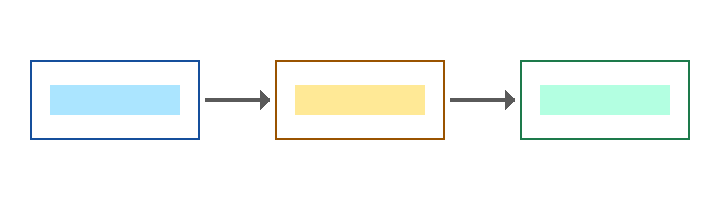
\includegraphics[width=0.6\linewidth]{figures/overview.png}
  \caption{Overview of \method{}. The retriever proposes candidate passages and the cross-encoder re-ranks them before generation.}
  \label{fig:overview}
\end{figure}

\section{Experiments}
We evaluate on three open-domain question answering datasets.
Table~\ref{tab:results} reports exact-match accuracy and the hallucination rate, which we measure as the fraction of answers that contain a claim not supported by the retrieved passages.

\begin{table}[t]
  \centering
  \begin{tabular}{lcc}
    \toprule
    Method & Exact match (\%) & Hallucination rate (\%) \\
    \midrule
    Closed-book model & 41.2 & 38.5 \\
    Standard RAG & 52.7 & 21.0 \\
    \method{} (ours) & 52.1 & 14.5 \\
    \bottomrule
  \end{tabular}
  \caption{Results averaged over the three benchmarks.}
  \label{tab:results}
\end{table}

\paragraph{Ablation.} Removing the cross-encoder increases the hallucination rate to 19.8\%, which shows that re-ranking is the main source of the improvement.
Increasing $k$ beyond 50 did not help, because the additional passages were rarely relevant.

\section{Conclusion}
Re-ranking retrieved evidence is a cheap and effective way to make generated answers more faithful.
Future work should study how the retriever and the generator can be trained jointly.

\bibliographystyle{plainnat}
\bibliography{refs}
\end{document}
